\documentclass[11pt]{article}

\usepackage[T1]{fontenc}
\usepackage{geometry}
\usepackage{amsmath, amssymb, amsthm}
\usepackage{listings}
% \usepackage{courier}
\usepackage{xcolor}
\usepackage{graphicx}
\usepackage{fancyhdr}
\usepackage{lipsum}
% \usepackage{subfigure}
\usepackage{caption}
\usepackage{subcaption}
\usepackage{float}
\usepackage{hyperref}

\makeatletter
\renewcommand\@biblabel[1]{}
\renewenvironment{thebibliography}[1]
     {\section*{\refname}%
      \@mkboth{\MakeUppercase\refname}{\MakeUppercase\refname}%
      \list{}%
           {\leftmargin0pt
            \@openbib@code
            \usecounter{enumiv}}%
      \sloppy
      \clubpenalty4000
      \@clubpenalty \clubpenalty
      \widowpenalty4000%
      \sfcode`\.\@m}
     {\def\@noitemerr
       {\@latex@warning{Empty `thebibliography' environment}}%
      \endlist}
\makeatother

% \captionsetup[table]{skip=10pt}

\geometry{a4paper, margin=1in, headheight=14pt}

\pagestyle{fancy}
\renewcommand\headrulewidth{0.4pt}
\fancyhead[L]{\scshape Experiment III}
% \lhead{Experiment I}
\rhead{}
\cfoot{\thepage}

\definecolor{darkgreen}{rgb}{0.2, 0.6, 0.4}
\definecolor{darkblue}{rgb}{0.2, 0.4, 0.8}
\lstset{ 
  basicstyle=\footnotesize\ttfamily,
  commentstyle=\color{gray},
  % extendedchars=true,
  % keepspaces=true,
  keywordstyle=\color{darkblue},
  % numbers=left,
  % numbersep=5pt,
  % numberstyle=\tiny\color{gray},
  stringstyle=\color{darkgreen},
  tabsize=4,
  % frame=lines,
  aboveskip=2em,
  belowskip=2em,
  breaklines=true
}

\newcommand\pp[2]{\frac{\partial #1}{\partial #2}}
\newcommand\E[1]{\langle #1 \rangle}

\title{
        \Large\textsc{PH2103: Physics Laboratory III} \\
        \vspace{10pt}
        \Huge \textbf{Interferometry and Coherence} \\
        \vspace{5pt}
        \large{Michelson's Interferometer and the refractive index of glass.}
}
\author{
        \large Satvik Saha%
        \thanks{Email: \tt ss19ms154@iiserkol.ac.in}
        \\\textsc{\small 19MS154}
}
\date{\normalsize
        \textit{Indian Institute of Science Education and Research, Kolkata, \\
        Mohanpur, West Bengal, 741246, India.} \\
        \vspace{10pt}
        \today
}

\begin{document}
        \maketitle

        % \renewcommand{\abstractname}{Aims}
        \begin{abstract}
                In this experiment, we employ division of amplitude interferometry in the form of Michelson's interferometer in order to
                determine the refractive index of glass.
                We also briefly discuss the concept of coherence.
        \end{abstract}

        \section{Theory}

        Interferometry is the technique of using the phenomenon of interference to extract information, such as lengths on a microscopic scale,
        or the speed of light through a given medium. There are two primary classes of interferometers -- division of wavefront and division
        of amplitude. We have already seen the former in the case of Young's Double Slit experiment. It is so named since a 
        wavefront is divided into two distinct point `sources' of coherent light, which recombine on a screen forming bands of dark and light
        lines called fringes. Division of amplitude interferometry is so called since a single beam is split into two beams at the same point in space,
        sent along different paths and recombined on a screen, forming linear or circular fringes. This is seen in the Michelson interferometer.
        It essentially consists of a source of monochromatic coherent light, a beamsplitter, two mirrors, and a screen. A slab of glass is
        often used as a compensator, which equalizes the optical path differences between the split beams.
        We use it here to control the path difference between the split beams, which can be used to measure the refractive index of the glass.

        \begin{figure}[H]
        \centering
                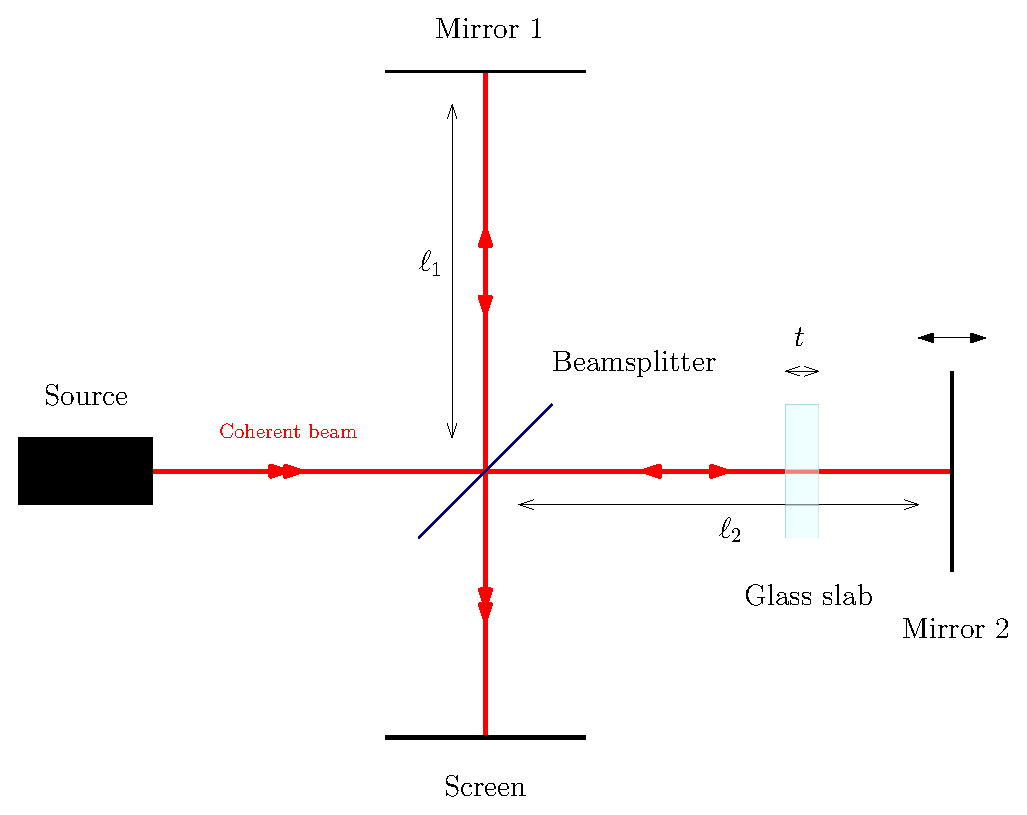
\includegraphics[scale=0.7]{./michelson.eps}
        \caption{Schematic of a Michelson interferometer, with a glass slab inserted in one end. In our experiment, we change the path difference
                between the arms by rotating this slab, instead of moving the second mirror.}
        \label{fig:michelson}
        \end{figure}

        As seen in Fig.~\ref{fig:michelson}, the two beams cover different optical path lengths.
        The beam striking mirror 1 covers a distance $2\ell_1$ between the split and the recombination.
        The other beam covers a distance $2(\ell_2 - t)$ in air, and $2t$ in glass. Setting the refractive index of glass as $n_g$,
        this corresponds to an optical path of $2(\ell_2 - t) + 2n_gt$. Note the factors of $2$, which arise because the beam travels to and back
        from the mirrors. The net optical path difference is thus $2\Delta\ell = 2(\ell_2 - \ell_1 + t(n_g - 1))$.
        The interference of these two beams with path difference $2\Delta\ell$ produces fringes on the screen.
        Note that the beams are actually spherical waves, so the path differences on the screen vary radially, producing circular fringes.
        Bright fringes are seen when the path difference is precisely an integer multiple of the wavelength $\lambda$ of the light used.
        The center of the screen, marked by a crosswire, is a bright spot only if $2\Delta\ell = n\lambda$, for integral $n$.
        
        Suppose that the path difference is changed by an amount $2d$. This can be done by moving one of the mirrors by $d$, or tilting the glass slab,
        effectively changing its thickness. This means that as the optical path difference at the center of the screen is changed
        from $2\Delta\ell \to 2\Delta\ell + 2d$, we move through several multiples of $\lambda$ in between, i.e.\ bright fringes are formed
        and disappear from the center. The entire diffraction pattern moves inwards/outwards, and the number of bright fringes which pass the center
        is given by the number of multiples of $\lambda$ in between the initial and final path differences, i.e.\ 
        \[
                d = \frac{m\lambda}{2}.
        \]

        \paragraph{Refractive index calculation}
        We know that a shift of $m$ fringes corresponds to a path difference of $m\lambda/2$.
        Consider a glass slab of thickness $t$, with its face initially normal to the light beam. We have already seen that this contributes
        a path length of $(n_g - 1)t$ (one way).

        \begin{figure}[H]
        \centering
                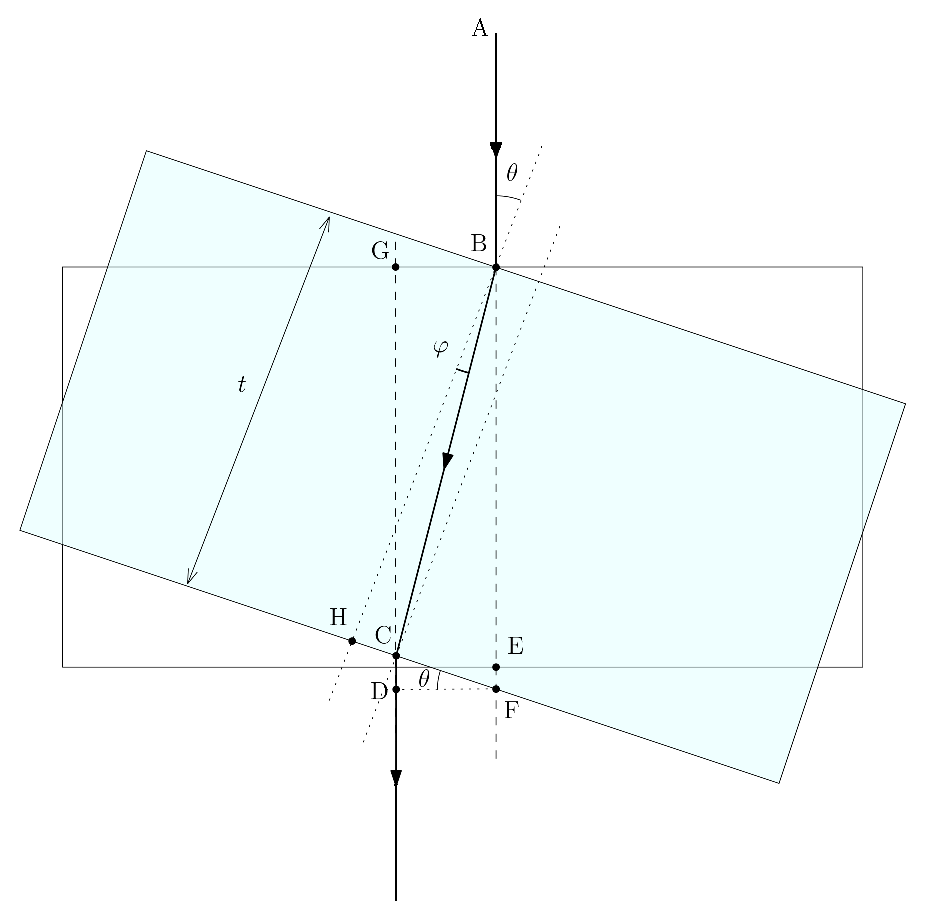
\includegraphics[scale=0.7]{./slab.eps}
        \caption{Schematic of the path followed by light through tthe rotated glass slab.}
        \label{fig:slab}
        \end{figure}

        Upon rotating the slab by $\theta$, light within the slab refracts and is deviated by an angle $\theta - \varphi$, where 
        $\sin\theta = n_g\sin\varphi$ by Snell's Law.
        The old optical path $n_g BE + EF$ has been replaced with $n_g BC + CD$.
        Simple geometry gives $BE = t$, $EF = BF - BE = t/\cos\theta - t$, $BC = t/\cos\varphi$ and 
        $CD = CF\sin\theta = (HF - HC)\sin\theta = t\tan\theta\sin\theta - t\tan\varphi\sin\theta$.
        Thus, the path difference is calculated as
        \begin{align*}
        n_g BC + CD - n_g BE - EF 
                        \;&=\; \frac{n_g t}{\cos\varphi} + \frac{t}{\cos\theta} + \frac{t\sin^2\theta}{\cos\theta} - 
                                \frac{t\sin\varphi\sin\theta}{\cos\varphi} - n_g t - \frac{t}{\cos\theta} + t \\
                        \;&=\; \frac{n_g t}{\cos\varphi}[1 - \cos\varphi - \sin\theta\sin\varphi /n_g] - 
                                \frac{t}{\cos\theta}[1 - \cos\theta - \sin^2\theta].
        \end{align*}
        Simplifying using Snell's Law and equating with the inferred path difference from $m$ fringe shifts, we obtain
        \[
                \frac{m \lambda}{2t} \;=\; (1 - \cos\theta) \,-\, n_g(1 - \cos\varphi).
        \]
        Rearranging,
        \[
                1 - \cos\varphi = \frac{1}{n_g}\left[1 - \cos\theta - \frac{m\lambda}{2t}\right] = \frac{\alpha}{n_g}.
        \]
        Now, this means that
        \[
                \cos^2\varphi = \left[1 - \frac{\alpha}{n_g}\right]^2 = 1 - \frac{2\alpha}{n_g} + \frac{\alpha^2}{n_g^2}.
        \]
        Using $\cos^2\varphi = 1 - \sin^2\varphi = 1 - \sin^2\theta /n_g^2$, we obtain $\sin^2\theta = 2\alpha n_g - \alpha^2$.
        Rearranging,
        \begin{align*}
                n_g \;&=\; \frac{\alpha^2 + \sin^2\theta}{2\alpha} \\
                        \;&=\; \frac{(1 - \cos\theta)^2 - 2(1 - \cos\theta)(m\lambda /2t) + (m\lambda /2t)^2 + \sin^2\theta}
                                        {2(1 - \cos\theta - (m\lambda /2t))} \\
                        \;&=\; \frac{1 - 2\cos\theta + \cos^2\theta + \sin^2\theta - 2(1 - \cos\theta)(m\lambda /2t) + (m^2\lambda^2/4t^2)}
                                {2(1 - \cos\theta - (m\lambda/2t))}.
        \end{align*}
        Thus,
        \[
                n_g \;=\; \frac{(1 - \cos\theta)(1 - m\lambda/2t) + m^2\lambda^2/{8t^2}}{1 - \cos\theta - m\lambda/2t}.
        \]
        For calculations, we can ignore the quadratic term, approximating
        \[
                n_g \;=\; \frac{(1 - \cos\theta)(1 - m\lambda/2t)}{1 - \cos\theta - m\lambda/2t}. \tag{$\star$}\label{eq:working}
        \]

        \subsection{Coherence}
        The formation of interference fringes relies on the fact that the path/phase differences between the interfering waves
        is well-defined and known at all points on the screen. If two waves are in phase at the source, we must be confident that
        they remain in phase at the beamsplitter, are precisely $2\Delta\ell \cdot 2\pi/\lambda$ out of phase after recombination, and remain
        so at the screen. In effect, given the phase relationship of a wavetrain at a particular point of time and space, we must be able to 
        say with confidence that this phase relationship is preserved over intervals of time and space.
        An ideal monochromatic, coherent light wave has an electric field of the form
        \[
                U(t) = A \cos(kx - \omega t).
        \]
        Note that this wave has exactly one frequency, $\omega$.

        In reality, this is not true -- waves are not generated as infinite wavetrains, but in bursts, which may remain correlated
        over the duration and length of the burst, but not between bursts. This means that after a certain distance, i.e.\ when the
        wave has traveled for a certain time, the phase relationship in the beam becomes completely uncertain. This length
        is called the coherence length $\ell_c$, and this time is called the coherence time $\tau_c$, related as $\ell_c = c\tau_c$.
        Thus, if the path length of light in our setup approaches and begins to exceed $\ell_c$, the fringes on the screen get washed out,
        eventually becoming unifrom. This is because the phase differences between waves at the screen essentially becomes random,
        so there are no particular regions where the intensities add up or cancel, hence no distinct maxima or minima.

        This leads to the idea of spatial and temporal coherence. Consider a beam of light with planar wavefronts.
        It is expected that over lengths of order $\ell_c$, these wavefronts will remain planar and maintain their shape. This
        is thus a measure of spatial coherence. It is also expected that the minima and maxima of the wavefront amplitudes
        will remain regular, i.e.\ equally spaced, over a time period $\tau_c$. This is a measure of the temporal coherence of the wave.

        To get a sense of scale for $\ell_c$, consider two wavetrains originating at the same point in space, of wavelengths $\lambda$ and
        $\lambda + \Delta\lambda$. Over short lengths, these appear to be identical, yet with distance, they fall out of phase.
        There will be a length $\ell$ where for the first time, the waves are exactly $\pi$ out of phase, i.e.\ they interfere destructively here.
        Suppose the first wave completes $n$ cycles here, so $\ell = n\lambda$. The second will only be halfway through the previous cycle,
        so $\ell = (n - 1 /2)(\lambda + \Delta\lambda)$. Equating these, we see that
        \[
                \ell_c \sim \ell \approx \frac{\lambda^2}{2\Delta\lambda}.
        \]
        
        A quasi-monochromatic, partially coherent wave has a spread of frequencies $\omega$. This means that its Fourier transform
        looks like a sharp, but finitely thick, peak centered at the mean frequency $\bar{\omega}$ and having a width of $\Delta\omega$,
        which is a measure of the spectral width, i.e.\ range of frequencies/wavelengths of the light, which in turn is inversely
        a measure of the temporal coherence. The larger the $\Delta\omega$, the more this peak lowers, broadens and flattens out.
        Such light remains partially coherent over lengths $\ell \gg 2\pi c/\bar{\omega}$, and $\ell \ll 2\pi c /\Delta\omega$.
        Note that $2\pi c /\bar{\omega}$ is essentially the average wavelength $\bar{\lambda}$ of the beam, and $2\pi c /\Delta\omega$ is a measure
        of the distance beyond which the waves fall out of phase.

        This is formalized by introducing the degree of temporal coherence $\gamma$ during interference calculations. Suppose two monochromatic waves 
        $E_1(t)$ and $E_2(t)$ fall on a scren. The intensity distribution on the screen at a particular point where the time difference is $\tau$
        is given by
        \[
                I = I_1 + I_2 + 2\Re \E{E_1^*(t) E_2(t + \tau)}.
        \]
        Here, $I_i = \E{|E_i(t)|^2}$. We define
        \[
                \gamma(t) = \frac{\E{E_1^*(t)E_2(t + \tau)}}{\sqrt{I_1I_2}} = |\gamma(\tau)|e^{i\alpha(\tau)}e^{-\bar{\omega}\tau}.
        \]
        Typically, $\alpha(\tau)$ changes much faster than $|\gamma(\tau)|$, so we approximate
        \[
                I = I_1 + I_2 + \sqrt{I_1I_2}|\gamma(\tau)|.
        \]
        The degree of coherence is related to the fringe visibility $\mathcal{V}$ as
        \[
                \mathcal{V} = \frac{I_{max} - I_{min}}{I_{max} - I_{min}} = \frac{2\sqrt{I_1I_2}}{I_1 + I_2}|\gamma(\tau)|.
        \]
        When $I_1 = I_2$, we have $\mathcal{V} = |\gamma(\tau)|$.
        Also note that in such a case,
        \[
                I_{max} = 2I[1 + |\gamma(\tau)|], \qquad
                I_{min} = 2I[1 - |\gamma(\tau)|].
        \]
        The factor $\gamma(\tau)$ is essentially a measure of the correlation between the two waves at a given point in space, also
        called the mutual coherence. When the beams are perfectly coherent, $|\gamma(\tau)| = 1$ and when they are perfectly incoherent,
        $|\gamma(\tau)| = 0$. The latter happens when $\tau \gg \tau_c$, so $\mathcal{V} = 0$.
        Typically, $|\gamma(\tau)|$ will decrease with increasing $\tau$, i.e.\ the fringe visbility decays with increasing path difference.


        In our setup, we have used a laser with a supposedly large coherence length, well beyond the tens of meters. Thus, we do not
        have to make any special adjustments to ensure that the path difference is low, and our observed fringes remain quite distinct.
        
        \section{Experimental setup}
        A Michelson interferometer is set up, much like in Fig.~\ref{fig:michelson}, with the glass slab on a rotational stage. The fringes
        as magnified using a lens. Now, the stage is rotated and the number of fringes shifted is counted as a function of the rotation angle $\theta$.
        Specifically, the angle $\theta$ is noted for fixed number of fringe shifts such as 20, 30, 40 and 50. This data is used
        to calculated $n_g$ using the working formula (\ref{eq:working}) as derived earlier.
        It is given that the wavelength of the laser $\lambda = 650$ nm, and the thickness of the glass $t = 1$ mm.

        \section{Experimental data and analysis}
        
        \subsection{Data processing}
        
        All data has been gathered into an Excel spreadsheet, read using \texttt{pandas} and processed using \texttt{numpy}.
        The code used has been listed below.

        \lstinputlisting[language=Python]{calculate.py}

        \subsection{Error Analysis}
        Set $\xi = \cos\theta$ and $\zeta = m\lambda / 2t$. Thus, using standard error propagation formulae, we have
        \[
                \left(\delta n_g\right)^2 \;=\; \left|\pp{n_g}{\xi}\right|^2(\delta\xi)^2 + \left|\pp{n_g}{\zeta}\right|^2(\delta\zeta)^2
                        \;=\; \left(\frac{\zeta(1 - \zeta)}{(1 - \xi - \zeta)^2}\right)^2(\delta\xi)^2 + 
                                        \left(\frac{\xi(1 - \xi)}{(1 - \xi - \zeta)^2}\right)^2(\delta\zeta)^2 .
        \]
        Now,
        \[
                \delta\xi = \left|\frac{\partial \xi}{\partial\theta}\right|\,\delta\theta = |\sin\theta|\,\delta\theta,
                \qquad\text{and}\qquad
                \left(\frac{\delta\zeta}{\zeta}\right)^2 = \left(\frac{\delta\lambda}{\lambda}\right)^2 + \left(\frac{\delta t}{t}\right)^2.
        \]
        The errors for $N$ such calculated values are averaged as $\delta n_g = \sqrt{\sum\delta n_{g, i}}$ for each set.
        This is done numerically with the aforementioned code.

        We have chosen $\delta\lambda = 3$ nm, $\delta\theta = 1^\circ = \pi/180$ rad, and $\delta t = 0.1$ mm. 
        Note that the standard deviations of $\theta$ for each $m$ are well within $1^\circ$ each.
        For each set, we also take the maximum of this propagated error and the standard deviation of the calculated values.

        \subsection{Tabulated data}

        \begin{table}[H]
                \centering
                \caption{Data from Set I.}
                \begin{tabular}{c|c|c|c}\hline
                Fringes shifted $m$&  Angle rotated $\theta^\circ$ &  Refractive Index $n_g$&     Propagated error \\\hline\hline
                    20 &            8.7 &          2.283473 &  0.741606 \\
                    20 &            9.4 &          1.925645 &  0.423516 \\
                    20 &            8.7 &          2.283473 &  0.741606 \\
                    20 &            8.6 &          2.354855 &  0.815078 \\
                    20 &            8.6 &          2.354855 &  0.815078 \\
                    20 &            8.7 &          2.283473 &  0.741606 \\
                    20 &            8.6 &          2.354855 &  0.815078 \\
                    \color{red}30 &           \color{red} 9.6 &       \color{red}   3.259884 &  \color{red}1.722282 \\
                    30 &           11.0 &          2.109946 &  0.493008 \\
                    30 &           11.7 &          1.865807 &  0.325026 \\
                    30 &           11.9 &          1.812576 &  0.292756 \\
                    30 &           11.9 &          1.812576 &  0.292756 \\
                    30 &           11.6 &          1.894715 &  0.343205 \\
                    30 &           12.4 &          1.701337 &  0.230382 \\
                    40 &           14.1 &          1.736125 &  0.226681 \\
                    40 &           12.8 &          2.069726 &  0.418611 \\
                    40 &           13.6 &          1.840182 &  0.280709 \\
                    40 &           12.7 &          2.106101 &  0.442821 \\
                    40 &           13.1 &          1.972179 &  0.356868 \\
                    40 &           12.7 &          2.106101 &  0.442821 \\
                    40 &           13.0 &          2.002920 &  0.375825 \\
                    50 &           15.0 &          1.880618 &  0.282957 \\
                    50 &           14.8 &          1.928176 &  0.308297 \\
                    50 &           15.1 &          1.858380 &  0.271455 \\
                    50 &           15.8 &          1.726177 &  0.207653 \\
                    50 &           15.4 &          1.797093 &  0.240903 \\
                    50 &           14.8 &          1.928176 &  0.308297 \\
                    50 &           16.0 &          1.694606 &  0.193577 \\
                \hline
                \end{tabular}
                \label{tab:data_1}
        \end{table}
        \begin{table}[H]
                \centering
                \caption{Data from Set II.}
                \begin{tabular}{c|c|c|c}\hline
                Fringes shifted $m$&  Angle rotated $\theta^\circ$ &  Refractive Index $n_g$&     Propagated error \\\hline\hline
                    20 &           11.5 &          1.469199 &  0.140328 \\
                    20 &           11.3 &          1.494670 &  0.152458 \\
                    20 &           11.4 &          1.481657 &  0.146206 \\
                    20 &           11.1 &          1.522506 &  0.166217 \\
                    20 &           11.5 &          1.469199 &  0.140328 \\
                    30 &           13.7 &          1.506533 &  0.137747 \\
                    30 &           13.5 &          1.530233 &  0.147881 \\
                    30 &           13.7 &          1.506533 &  0.137747 \\
                    30 &           13.6 &          1.518160 &  0.142679 \\
                    30 &           13.5 &          1.530233 &  0.147881 \\
                    40 &           15.3 &          1.558726 &  0.146858 \\
                    40 &           15.5 &          1.536048 &  0.137777 \\
                    40 &           15.8 &          1.504755 &  0.125666 \\
                    40 &           15.5 &          1.536048 &  0.137777 \\
                    40 &           15.4 &          1.547193 &  0.142208 \\
                    50 &           17.4 &          1.525469 &  0.125831 \\
                    50 &           17.2 &          1.545219 &  0.133074 \\
                    50 &           17.6 &          1.506861 &  0.119170 \\
                    50 &           17.3 &          1.535195 &  0.129375 \\
                    50 &           17.8 &          1.489304 &  0.113029 \\
                \hline
                \end{tabular}
                \label{tab:data_2}
        \end{table}
        \begin{table}[H]
                \centering
                \caption{Data from Set III.}
                \begin{tabular}{c|c|c|c}\hline
                Fringes shifted $m$&  Angle rotated $\theta^\circ$ &  Refractive Index $n_g$&     Propagated error \\\hline\hline
                    20 &            8.8 &          2.218503 &  0.677627 \\
                    20 &            8.6 &          2.354855 &  0.815078 \\
                    20 &            8.9 &          2.159131 &  0.621570 \\
                    30 &           10.4 &          2.435918 &  0.768221 \\
                    30 &           10.8 &          2.202763 &  0.565452 \\
                    30 &           10.5 &          2.370494 &  0.708326 \\
                    40 &           12.7 &          2.106101 &  0.442821 \\
                    40 &           12.9 &          2.035387 &  0.396347 \\
                    40 &           12.6 &          2.144694 &  0.469212 \\
                    50 &           14.8 &          1.928176 &  0.308297 \\
                    50 &           14.2 &          2.101284 &  0.409060 \\
                    50 &           15.1 &          1.858380 &  0.271455 \\
                \hline
                \end{tabular}
                \label{tab:data_3}
        \end{table}

        \subsection{Reported Values}
        We report the following refractive indices, standard errors and percentage errors for each of the three sets.
        \begin{center}
                \begin{tabular}{lcr}
                        Set I   & $2.03 \;\pm\; 0.31$ & 15\%\\
                        Set II  & $1.52 \;\pm\; 0.03$ &  2\%\\
                        Set III & $2.16 \;\pm\; 0.17$ &  8\%
                \end{tabular}
        \end{center}
        It is clear that the refractive index from set I and II agree with each other, but disagree with the value from set II.
        Despite having the largest number of measurements, set I has a very high standard error of $0.3$. This is likely because of
        the datapoint marked in red in Table~\ref{tab:data_1}.
        
        \section{Discussion}
        
        \subsection{Sources of error}
        The greatest contributer of measurement error is the angle measurement, which seems to have a fairly large range for a given fringe shift.
        The errors due to the wavelength and thickness of the slab are practically negligeable.

        Systematic error may arise from an incorrectly calibrated angle measurement, i.e.\ the laser may not be perfectly normal to the 
        slab face at $\theta = 0$. The glass slab might also not be perfectly cut or may be inhomogeneous, although these errors are probably 
        too small to have any effect.
        
        \subsection{Measurement of coherence length}
        In order to measure the coherence length of the laser beam, we dispense with the glass slab and seek the path difference $2\Delta\ell$
        at which the fringe visibility $\mathcal{V}$ becomes zero, i.e.\ the fringes lose all contrast. We must also choose the path
        difference such that if it were any shorter, the fringes appear again.
        At such a path difference, i.e.\ the maximum path difference at which fringes are still visible, we may conclude that $\ell_c \approx 2\Delta\ell$.
        Now, we know that $\ell_c$ for a laser is typically very high, so merely extending one arm even across a room while leaving the other 
        in place may not produce a high enough $\Delta\ell$. 
        Introducing a thick glass slab does increase the path length, but perhaps by an insufficient amount, only by $2(n_g - 1)t$.
        Thus, we propose taking the beam from one of the arms and reflecting it back and forth several times across two mirrors facing each other 
        before returning it to the beamsplitter. This is difficult, as it requires keeping count of the number of reflections.
        Suppose the light beam is allowed to bounce between two parallel mirror planes of length $L$ separated by a distance $d$, 
        in a way that it enters this arrangement at an angle $\beta$ from the mirror planes.
        Thus, when light bouncing off the mirrors has travelled the entire length $L$, it has covered a distance $L /\cos\beta$.
        By increasing $\beta$ closer and closer to $\pi /2$, we can thus increase the path length arbitrarily. Once the beam reaches the other
        end, we can send it back along the same path with the original `Mirror 1'.

        \section{Conclusion}
        In conclusion, we have observed the phenomenon of interference via division of amplitude, and used this to calculate the refractive
        index of glass. We have also discussed the phenomenon od coherence in this context.

        \nocite{*}
        \bibliographystyle{plain}
        \bibliography{ref}

\end{document}
